%!TeX spellcheck = en-US
\chapter{Introduction}\label{cha:Introduction}
Technology is integrating more and more into the life of the modern man. A very important
question is how are people interacting with technology.
The human brain does not react emotionally to artificial objects like computers and
mobile phones. However, the human brain reacts strongly to human appearances like
the shape of the human body or faces. Therefore humanoid robots are the most
natural way for human-machine interaction, because of the human-like appearance.
This hypothesis is strongly supported by Takayuki Kanda and Hiroshi Ishiguro in \cite{kanda2017human}.
They see Social Robots as a part of the future society as shown in figure \ref{fig:socialRobotsFuture}.
\begin{figure}
  \centering
  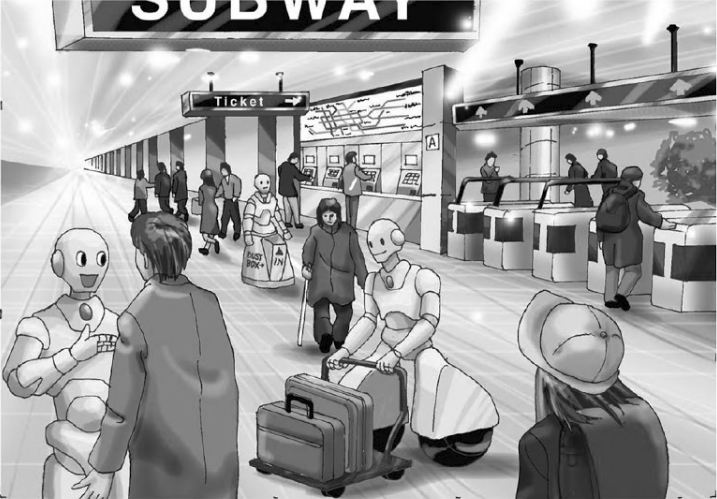
\includegraphics[width=.6\textwidth]{socialRobotsFuture.png}
  \caption{Social Robots in the future society \cite{kanda2017human}}
  \label{fig:socialRobotsFuture}
\end{figure}
Takayuki Kanda and Hiroshi Ishiguro also define the following three issues which
need to be solved to bring social robots effectively and safely to the everyday life:
\begin{itemize}
  \item [a.] Sensor network for tracking robots and people
  \item [b.] Development of humanoids that can work in the daily environment.
  \item [c.] Development of functions for interactions with people.
\end{itemize}
This thesis is located in the field \texttt{c}, as we try to implement a Visual Voice Activity Detection (VVAD) which detects whether a person is speaking to a robot or not, given the visual input of the robot's camera. The detailed description of the problem
setting is given in Section \ref{sec:problem}.


\section{Motivation}\label{sec:motivation}
In this Section we want to present why a VVAD is an important cognitive feature in a Human-Robot Interaction(HRI).
As we want Robots to integrate seamlessly into our society, Human-Robot Interaction needs to be as close as possible to Human-Human Interaction(HHI). To achieve this goal we need to understand how humans communicate.
In specific we need to know how humans start a conversation.
There is one main concept when it comes to starting an interaction, which is deeply encoded in our DNA, as it is used by newborns and even animals follow this concept. To start a interaction of any kind one needs to increase the attention of the other. In HHI an increased attention comes mainly from the following stimuli:
\begin{itemize}
  \item {1.} auditory stimuli
  \item {2.} tactile stimuli
  \item {3.} visual stimuli
\end{itemize}
In the context of a conversation all the above stimuli can represent a direct starting point to a conversation.
For auditory stimuli a direct starting point can be a name or a word socially known to increase attention
like \emph{hey} in the English language. Calling someones name works like a directed message to someone, while words like \emph{hey} work like a broadcast to everyone in the surrounding. The concept of using names as a trigger phrase for virtual assistant systems is implemented in well known assistants like the Amazon Alexa, the Google Assistant or Apples Siri.

A tactile stimulus gives direct attention because the human body is very sensitive to tactile stimuli in a way that every individual has it's own private space. A tactile stimulus is invading a humans personal space and is therefore triggering an increase in attention. Meaning when you touch someone and say something directly afterwards the touched person can directly process the message, because of the increased attention.

For visual stimuli gaze and eye contact have been studied for decades, because they have such a special role in HHI. As Michael Argyle and Janet Dean stated in \cite{ARGYLE1965} gaze has a huge influence on the personal space and therefore also increases the attention. Meaning if eye contact is established and one of the two parties speaks it works like a directed message.


As the hypothesis of Takayuki Kanda and Hiroshi Ishiguro is that humans will react more naturally to human-like robots, it is obvious that not only the physical appearance needs to be human-like, also the psychological concepts of interaction need to be implemented.

For the purpose of this thesis we want to enhance the implementation of a Pepper Robot from SoftBank Robotics Group Corp.(a detailed description of the robot can be seen in Appendix \ref{sec:pepper}).\footnote{All further mentions of \emph{the robot} refer to the Pepper Robot}
The robot already is able to react to the described stimuli. Nevertheless there is a gap after that.
Assuming someone is establishing eye contact with the robot.
Which will result in an increase of the robots attention, meaning he will start listening.
But the problem here is that the robot does not have the capability to detect if the person, eye contact is established with, is speaking.
The robot may respond to something someone else in the surrounding was saying, which will confuse the person, eye contact is established with, and result in a non natural way of communication.
To solve this problem we want to develop a VVAD which detects whether a person is speaking to a robot or not, given the visual input of the robot's camera. Thus the robot can decide whether to listen if the person is speaking to it or to proactively act on the invasion of it's personal space if the person is just starring at the robot.
We hope that this social skill will improve the quality of HRI in a way that communicating with a robot feels more natural.




\section{Problem Setting}\label{sec:problem}

As stated before this thesis deals with the implementation of a VVAD which detects whether a person is speaking to a robot or not, given the visual input of the robot's camera.
We consider an open world setting in which people start an interaction with the robot whenever they want and it can also occur that people are talking near the robot without talking directly to the robot.
In such an environment the robot should be able to react on a visual stimulus (described in Section \ref{sec:motivation}) as natural as possible.
The algorithm to classify whether a person is just starring at the robot or is speaking to the robot will be performed solely on video data from the camera of the robots head. This seems to be unnecessary few input on first sight, as the robot provides a lot more useful information, like audio input and even echo location. But with a closer look to the described cognitive feature of detecting an invasion of personal space on the basis of visual stimuli, it is only logical to reduce the input to only visual information. A fusion of different cognitive features could happen on a higher level of cognition.
As described in Section \ref{sec:motivation} we use a Pepper Robot as the target platform. Pepper provides video data in a maximum resolution of 2592x1944 pixels at a framerate of 1 fps or with a maximum framerate of 30 fps with a resolution of 640x480 pixels(for further details of the given Hardware see Appendix \ref{sec:pepper} and \cite{Pepper2018}).


\section{Approach}\label{sec:approach}
%(taking the 30 fps)
%training data
%RNN
%different modeling approaches
% 1. Feature reduction(relative postion?)
%  1.1 only mouth features
%  1.2 whole face features
% 2. Direct Learning(name?)
%  2.1 only mouth image
%  2.2 whole face image
In this Section we will describe the approach to develop a VVAD which detects whether a person is speaking to a robot or not, given the visual input of the robot's camera. This goes from the training data over the learning algorithm to the evaluation.
\subsection{Training data}\label{ssec:data}
To train our classifier we need a dataset which has labeled video data. As we try to solve a binary classification problem the data needs to have two labels. In our case these would be \emph{speaking} as the positive class and \emph{not speaking} as the negative class on every sample of the dataset. We also need a Region of Interest (ROI) on every image. So we end up with samples, that are labeled video sequences of faces either \emph{speaking} or \emph{not speaking}.
The University of Oxford developed three datasets(LRW, LRS2, LRS3) for lipreading in cooperation with the BBC and TED \cite{Chung16}, \cite{Chung17},\cite{Chung18}. These need to be slightly adjusted to the purpose of the thesis. The video data is labeled with words and the corresponding timestamps. It also provides a face bounding box for every frame.
The positive class can be easily extracted from this datasets, as we know which frames correspond to speech.
The negative class needs to be extracted from the phases where the person is not speaking, which can be slightly more challenging because the phases are not stored in the dataset's labels. As we know there is no speech in those phases we follow the given face from the ROI to construct a negative sample if the number of frames is over a given threshold.

\subsection{Learning algorithm}\label{ssec:algorithm}
To choose a good fit for the learning algorithm it is important to exploit the knowledge of the underlying data. In the case of a VVAD, we are dealing with sequences of video frames.
%Following \cite{Zhengzheng2010} a sequence can be described as follows:
%\begin{itemize}
%\item[•] Given an alphabet of symbols  $\left\lbrace E_1, E_2, E_3, ..., E_n \right\rbrace$, a
%\emph{simple symbolic sequence} is an ordered list of the symbols
%from the alphabet. For example, a DNA sequence
%is composed of four animo acid A, C, G, T and a DNA
%segment, such as ACCCCCGT, is a simple symbolic
%sequence.
%\item[•] A \emph{complex symbolic sequence} is an ordered list of vectors.
%Each vector is a subset of the alphabet \cite{Lesh99}. For
%example, for a sequence of items bought by a customer
%over one year, treating each transaction as a
%vector, a sequence can be $\left\langle (milk, bread)(milk, egg)\cdots(potatos, cheese, coke)\right\rangle$.
%\item[•] A \emph{simple time series} is a sequence of real values ordered
%in timestamp ascending order. For example, $\left\langle(t_1, 0.1)(t_2, 0.3)\cdots(t_n, 0.3)\right\rangle$
%is a simple time series recording the data from time
%stamp $t_1$ to $t_n$.
%\item[•] A \emph{multivariate time series} is a sequence of numerical
%vectors. For example,
%
%$\left\langle (t_1,\left\langle 0.1, 0.3, 05\right\rangle )(t_2,\left\langle 0.3, 0.9, 0.8\right\rangle )\cdots(t_n,\left\langle 0.3, 0.9, 0.4\right\rangle )\right\rangle $
%is a multivariate time series.
%\item[•] In the above, the data types of the events are simple.
%In some applications, the data type of events can be arbitrarily
%complicated. For example, in a patient record
%data set (\url{http://www.informsdmcontest2009.org/}),
%each patient is represented by a longitudinal sequence
%of hospital visits. Each visit is an event and is described
%by multiple numerical measurements, categorical
%fields and text descriptions. A \emph{complex event sequence}
%refers to the general form of sequences.
%\end{itemize}
As described in Section \ref{ssec:data} every sample is annotated with a positive (\emph{speaking}) or a negative (\emph{not speaking}) label $y$ and is described by a  ROI as a face bounding box from which we can extract a vector of features(these can be the pixels directly or features from the face detection) $\mathbf{x} = \left\langle x_{0}, x_{1}, \cdots , x_{n-1}, x_{n} \right\rangle$. What we want is a classifier that maps a sequence of those frames to a class.
\begin{equation}\label{eq:classifier}
f: \left\langle \mathbf{x}_{t}, \mathbf{x}_{t-1}, \cdots, \mathbf{x}_{t-k} \right\rangle \rightarrow y_{t} \quad |\ y \in \left\lbrace0,1\right\rbrace,\ k \in \mathbb{N}\ |\ 0<k\leq t
\end{equation}
This classifier uses a temporal sliding window, to always perform the classification on the last $k$ frames. The hyperparameter $k$ needs to be chosen  small enough to make the classification fast enough, but needs to be chosen big enough to secure accuracy.
For $\mathbf{x}$ we will evaluate four different approaches.
These can be split in $2 \times 2$ categories. The first categories are \emph{Focus on facial features} or \emph{End-to-End Learning}.
The second categories are \emph{only mouth} or \emph{whole face}.
This will end up in the following four models, which should be tested against each other:
\begin{itemize}
  \item Focus on facial features
  \begin{itemize}
  	\item only mouth features
  	\item whole face features
  \end{itemize}
  \item End-to-End Learning
  \begin{itemize}
  	\item only mouth image
  	\item whole face image
  \end{itemize}
\end{itemize}
For the facial features we want to use dlib's\cite{Dlib} pretrained Convolutional Neural Network (CNN) for face shape detection which gives 68 features for a face including 20 features for the mouth.
Independent of which model we use, we will need to apply some kind of normalization to the scale, rotation and translation of the features. The face or the mouth can appear in any translation, rotation and scale in the dataset, with the normalization we make sure that we concentrate on the important features of the image. Otherwise it could happen, that the classification is based on the position of the face in the image, which is obviously not correct.
As we want to know the label for a ongoing sequence as fast as possible it is considered to be a problem of early classification of time series
data \cite{Xing2011}. As described earlier we use a fixed size temporal sliding window to solve this issue.
Our approach to solve the classification problem is a Long Short Term Memory (LSTM) Fully Convolutional Network (FCN).
As shown in \cite{Fazle18} \cite{Fazle17} Recurrent Neural Networks (RNNs) and in specific LSTM-FCNs are the state of the art method for Time Series Classification.

\subsection{Evaluation}\label{ssec:evaluation}
To evaluate the classification we will use a dedicated test set created with the extraction of the samples from the LRS3 dataset. 
For this test set a human accuracy level test is conducted to evaluate the results from a test on that specific test set. 
Furthermore the human accuracy level test can give information about the quality of the constructed dataset.
The evaluation is performed on the described four different learning approaches in terms of the input features described in Section \ref{ssec:algorithm}. 

\section{Related Works}\label{sec:relatedWorks}
The classic approach to solve Visual Voice Activity Detection is to detect lip motion.
This approach is taken by F. Luthon and  M. Liévin in \citep{Luthon1998}. They try to model the motion of the mouth in a sequence of color images with Markov Random Fields. For the lip detection they analyze the images in the \emph{HIS ( Hue,
Intensity, Saturation )} color space, with extracting \emph{close-to-red-hue prevailing regions} this leads to a robust lightening independent lip detection.
A different approach was taken by Spyridon Siatras, Nikos Nikolaidis, and Ioannis Pitas in \cite{Siatras2006}. They try to convert the problem of lip motion detection into a signal detection problem. They measure the intensity of pixels of the mouth region and classify with a threshold, since they argue that frames with an open mouth have a essentially higher number of pixels with low intensity.
In \citep{Bendris2010} Meriem Bendris, Delphine Charlet and Gérard Chollet propose a method,
which measures the probability of voice activity with the optical flow of pixels in the mouth region. In this paper the drawback of lip motion detection based approaches is already discussed.
As shown in Figure \ref{fig:errorDetection} the problem is that people move their lips from time to time although they are not speaking.

\begin{figure}
\centering
  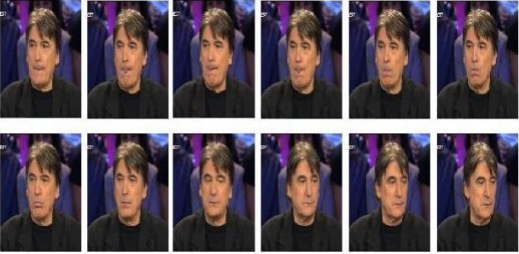
\includegraphics[width=.75\textwidth]{error_detection.png}
  \caption{Example of error detection - Person is classified as
having a mouth activity, however does not speak \cite{Bendris2010}}
  \label{fig:errorDetection}
\end{figure}

This issue is tackled by Foteini Patrona, Alexandros Iosifidis et al. \cite{Patrona2016}.
They use a Space Time Interest Point(STIP) or the Dense Trajectory-
based facial video representation to train a Single Hidden Layer Feedforward Neural Network.
The features are generated from the CUAVE dataset \cite{Patterson2002}.
This erases the implicit assumption (of the approaches above) that lip motion equals voice activity.
A more robust approach, which uses Centroid Distance Features of normalized lip shape to train a LSTM Recurrent Neural Network is proposed by Zaw Htet Aung and Panrasee Ritthipravat in \cite{Aung2015}. This method shows a classification accuracy up to 98\% on a relatively small dataset.
In conclusion all of the mentioned methods use some kind of face detection and some also use mechanics to track the face. This is needed if there is more than one face in the image.
From the facial images features are created in different ways. From that point the approaches divide into two branches.
The first and naive approach is to assume that lip motion equals speech. This is obviously not always the case, which is why the later approaches do not rely on this hypothesis.
The latter approach uses learning algorithms to learn the real mapping between facial images and the speech/no speech. This approach is strongly relying on a balanced dataset to learn a good performing model.

\section{Software}
\label{sec:software}
In larger projects, independent if its software, hardware or even something else, it makes sense to
take advantage of the knowledge of others.
In terms of software this can be very easy, because the Internet is full of libraries, that provide solutions for various problems.
The few used to implement the VVAD are presented in the following.
\subsection{Keras}
To design the Deep Neural Networks used to make the prediction for the VVAD \emph{Keras}\cite{Keras} is used.
Keras is a python library which provides a high-level API(Application Programming Interface) for Artificial Neural Networks. It is designed to run on top of TensorFlow, CNTK or Theano and abstracts their implementation to a easy to use API for Deep Learning. 
It supports computation on CPU and GPU.
\subsection{NumPy}
\emph{NumPy}\cite{NumPy} is the go to library for scientific computations in python.
It provides powerful computation in linear algebra due to its C++ implementation. 
NumPy is used to transform all data into the shape needed by Keras and to produce meaningful visualizations of the data.  
\subsection{Dlib}
\emph{Dlib}\cite{Dlib} is a C++ library with very good python bindings which provides a lot of machine learning and image processing algorithms.
Dlib's face detection, tracking and facial landmark detection is used to construct the VVAD dataset from the LRS3 dataset.
\subsection{OpenCV}
Similar to Dlib, \emph{OpenCV}\cite{OpenCV} is a C++ implementation with strong python bindings. 
OpenCV provides a great variety of algorithms from the field of computer vision.
It is used for its very efficient basic operations on images, like loading, resizing and transformation to different color spaces.
\subsection{Express}
\emph{Express}\cite{EXPRESS} is a NodeJS library which provides a high-level API for the design of web apps.
Express is used for the Human Accuracy Level Test described in Section \ref{ssec:VVADHACL}.
\subsection{MongoDB}
\emph{MongoDB}\cite{MONGO} is a cross-platform document-oriented NoSQL database, which is used to store the classifications made in the Human Accuracy Level Test.

\section{Contribution}
In this thesis the problem of VVAD is defined and a large scale dataset called the \emph{VVAD dataset} (see Section \ref{sec:vvadData}) is constructed for this purpose.
The results obtained in this thesis using the proposed different approaches define the state of the art for VVAD problem.
Table \ref{tb:accuracies} shows an overview of the accuracies reached by the different approaches.


%\section{Time table}
%
%\begin{ganttchart}[vgrid={draw=none, dotted}]{1}{24}
%\gantttitle{Weeks}{24} \\
%\gantttitlelist{1,...,24}{1} \\
%\ganttbar{Literature Research}{1}{5} \\
%\ganttbar{Data acquisition}{3}{7} \\
%\ganttbar{Implementing models}{7}{16} \\
%\ganttbar{Tuning models}{16}{19} \\
%\ganttbar{Evaluation}{19}{23} \\
%\ganttbar{Writing thesis}{3}{24}
%\end{ganttchart}


%\begin{ganttchart}[vgrid={draw=none, dotted}]{1}{24}
%\gantttitle{Weeks}{24} \\
%\gantttitlelist{1,...,24}{1} \\
%\ganttbar{Literature Research}{1}{5} \\
%\ganttbar{Data acquisition}{3}{7} \\
%\ganttbar{Implementing models}{7}{16} \\
%\ganttbar{Tuning models}{16}{19} \\
%\ganttbar{Evaluation}{19}{23} \\
%\ganttbar{Writing thesis}{3}{24}
%\end{ganttchart}
%
%\begin{figure}[H]
%\centering
% % \includegraphics[width=\textwidth]{Gantt.png}
%
%  \caption{The approximate time table for the completion of the thesis}
%  \label{fig:Gantt}
%\end{figure}


%\section{Preliminaries}\label{sec:preliminaries}
% TODO: Write intro to this see liu-kappas
%\subsubsection{Thin-slicing}\label{subsec:thin-slicing}
% TODO: Write text see liu-kappas
%\subsection{Artificial Neural Networks(ANNs)}
%TODO: write from input of the deep learning book
